%% 
%%	This is file 'beamer_sample.tex'
%%	according to an MPIDR's PowerPoint template (?)
%%	
%%	by Eric Naujoks
%%
%%	Problems, bugs and comments to 
%%	naujoks@demogr.mpg.de
%%

%%%%%%%%%%%%%%%%%%%%%%%%%%%%%%%%%%
%%	Praelegomena								%%
%%%%%%%%%%%%%%%%%%%%%%%%%%%%%%%%%%
%%	- Make sure that you use utf8-encoding for all your .tex-files!!! (TeXnicCenter since version 2.0)
%%	- TeXnicCenter update: MPIDR intranet > Hard- & Sortfware > Software > Script and text editors > TeXnicCenter

\documentclass[20pt]{beamer}

\usepackage[ngerman,english]{babel}
\usepackage{tikz}
\usepackage[normalem]{ulem}
\geometry{paperwidth=10in, paperheight=7.5in}
\usepackage{animate}

\usepackage[utf8]{inputenc}

\usepackage[mpidr]{./mpidr/beamerthemeMPIDR}

%% Declaring title and author
\title{A unified framework\\ of demographic time}
\subtitle{Tim Riffe \\ Jonas Sch{\"o}ley \\ Francisco Villavicencio}		%%

%%	the institute's logo
\renewcommand{\mylogo}{\includegraphics[width=4.7in]{mpidr_logo_colour_en}}
\usepackage{color}
\definecolor{mygray}{rgb}{0.8,0.8,0.8}

\defbeamertemplate{description item}{align left}{\insertdescriptionitem\hfill}
%%	should be the very last package to be loaded
\usepackage{hyperref}

%%%%%%%%%%%%%%%%%%%%%%%%%%%%%%%%%%
%%	Beginning of the document		%%
%%%%%%%%%%%%%%%%%%%%%%%%%%%%%%%%%%
\begin{document}

%%	titlepage - fixed frame:
%%	========================

\begin{frame}
	\titlepage
\end{frame}
%-------------------
\begin{frame}
\frametitle{Demographic time}
% three stock images: baby, clock or timeline, death (scythe?)
\end{frame}
%-------------------
\begin{frame}
\frametitle{Demographic time measures}
%%%%%%%%%%%%%%%%%%%%%%%%%%%%%%%%%%
% 1) make graphics appear when line comes to foreground.
% 2) maybe description list type so that letters can be normal bold
%%%%%%%%%%%%%%%%%%%%%%%%%%%%%%%%%%
\begin{itemize}[<+->]
  \item \texttt{P}: 
\includegraphics[scale=.5]{Figures/llP.pdf} 
  \hspace{2em}period, calendar year
  \item \texttt{A}: \includegraphics[scale=.5]{Figures/llA.pdf}
  \hspace{2em}chronological age
  \item \texttt{C}: \includegraphics[scale=.5]{Figures/llC.pdf}
  \hspace{2em}birth cohort
  \item \texttt{T}: \includegraphics[scale=.5]{Figures/llT.pdf}
  \hspace{2em}thanatological age (TTD)
  \item \texttt{D}: \includegraphics[scale=.5]{Figures/llD.pdf}
  \hspace{2em}death cohort
  \item \texttt{L}: \includegraphics[scale=.5]{Figures/llL.pdf}
  \hspace{2em}ultimate complete lifespan
\end{itemize}
\end{frame}


%------------------------

\begin{frame}
\begin{block}{objective}
We add a third dimension to the Lexis diagram to account for time-to-death. This
results in three \textit{new} kinds of 2D Lexis diagrams, and a 3D Lexis diagram
that is the intersection of the four \textit{degenerate} diagrams.
\end{block}
\color{mygray}(It turns out Lexis himself did something eerily similar, but not
identical. Happy to explain how it works too)
\end{frame}
%-------------------

\begin{frame}
\frametitle{The APC demographic time identity}
\vspace{-4em}
\begin{center}
\includegraphics[scale=1.7]{Figures/APCid.pdf}
\end{center}
\end{frame}

%-------------------

\begin{frame}
\frametitle{APC diagram (Lexis diagram)}
\begin{center}
\includegraphics[trim= 200 200 200 200, scale=1.5]{Figures/APCrt.pdf}
\end{center}
\end{frame}

%-------------------

\begin{frame}
\frametitle{The TAL demographic time identity}
\vspace{-4em}
\begin{center}
\includegraphics[scale=1.7]{Figures/TALid.pdf}
\end{center}
\end{frame}

%-------------------

\begin{frame}
\frametitle{TAL diagram}
\begin{center}
\includegraphics[scale=1.1]{Figures/TALrt.pdf}
\end{center}
\end{frame}

%-------------------

\begin{frame}
\frametitle{The TPD demographic time identity}
\vspace{-4em}
\begin{center}
\includegraphics[scale=1.7]{Figures/TPDid.pdf}
\end{center}
\end{frame}

%-------------------

\begin{frame}
\frametitle{TPD diagram}
\begin{center}
\includegraphics[trim= 200 200 200 200, scale=1.5]{Figures/TPDrt.pdf}
\end{center}
\end{frame}

%-------------------

\begin{frame}
\frametitle{The LCD demographic time identity}
\vspace{-4em}
\begin{center}
\includegraphics[scale=1.7]{Figures/LCDid.pdf}
\end{center}
\end{frame}

%-------------------

\begin{frame}
\frametitle{LCD diagram}
\begin{center}
\includegraphics[trim= 200 200 200 200, scale=1.5]{Figures/LCDrt.pdf}
\end{center}
\end{frame}

%-------------------

\begin{frame}
\frametitle{Four demographic time identities}
\vspace{-4em}
\begin{center}
\begin{tabular}{c c}
     \includegraphics[scale=.8]{Figures/APCid.pdf} &
     \includegraphics[scale=.8]{Figures/TALid.pdf} \\
     \includegraphics[scale=.8]{Figures/TPDid.pdf} &
     \includegraphics[scale=.8]{Figures/LCDid.pdf}    
\end{tabular}
\end{center}
\end{frame}


\begin{frame}
\frametitle{\textit{The} demographic time identity}
\vspace{-4em}
\begin{center}
\includegraphics[scale=1.7]{Figures/TetraHedronEdgesOnly.pdf}
\end{center}
\end{frame}

%-------------------

% build this sequentially.
% 1) vanishing lines
% 2) APC laid flat in final position (years and ages labelled)
% 3) Year 2000 TAL plane sits on top (thano age labelled)
% 4) then complete diagram.
% CAN this all be done in Inkscape without needing to remake everything?

%-------------------
\begin{frame}
\frametitle{Building the demographic time diagram (1)}
\vspace{-1em}
\begin{center}
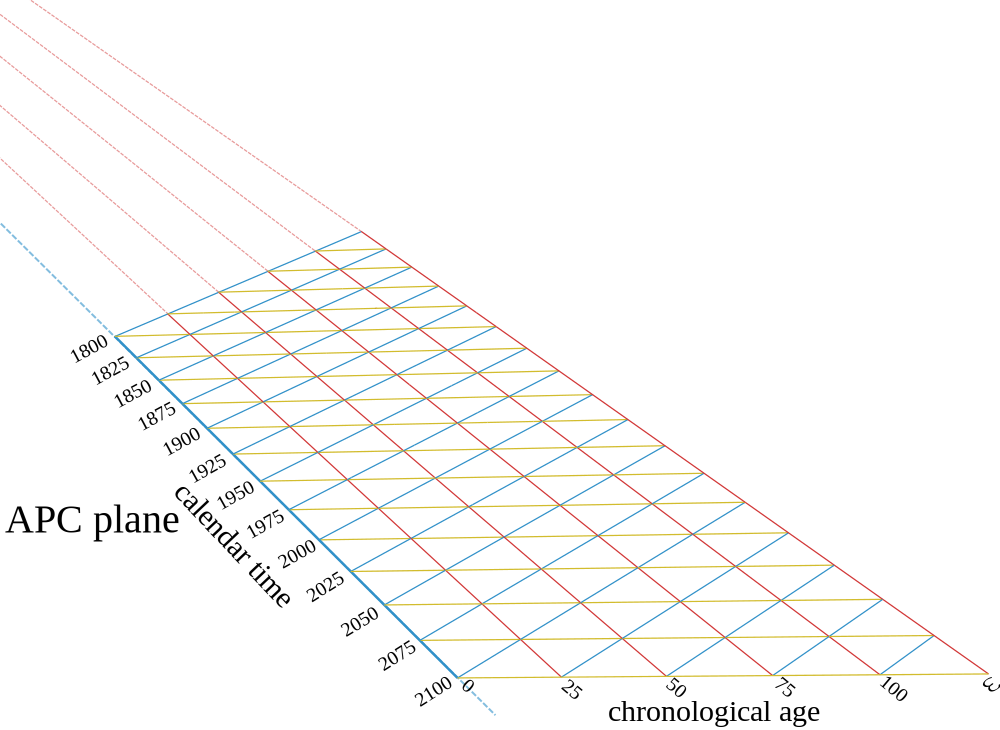
\includegraphics[scale=.8]{Figures/buildTAL1.pdf}
\end{center}
\end{frame}
%-------------------
\begin{frame}
\frametitle{Building the demographic time diagram (2)}
\vspace{-1em}
\begin{center}
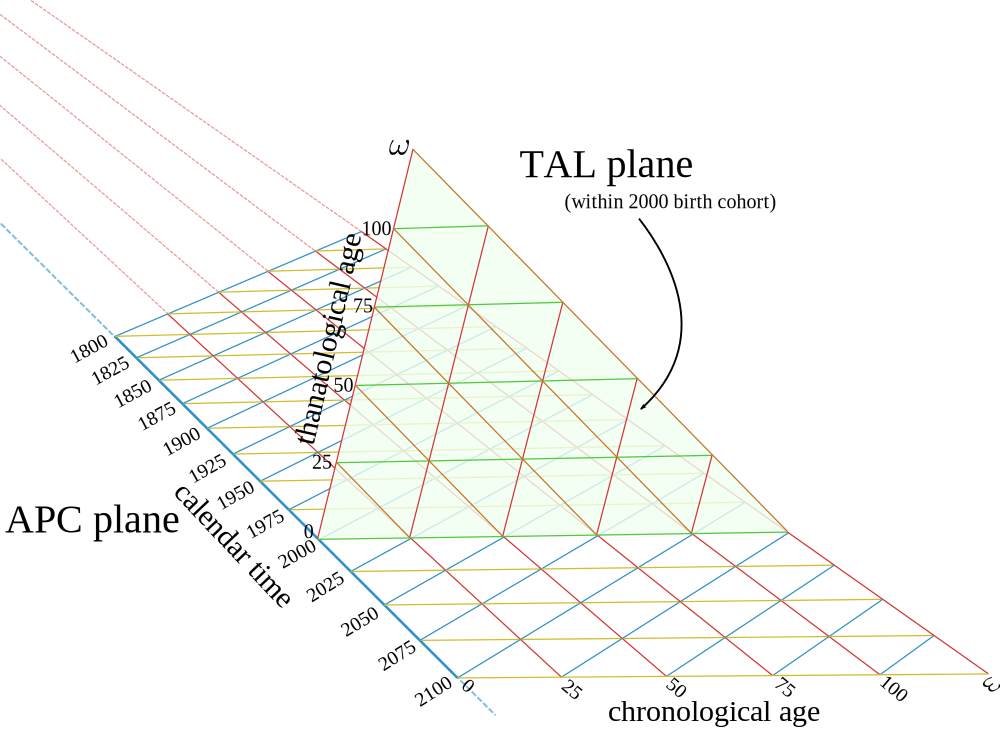
\includegraphics[scale=.8]{Figures/buildTAL2.pdf}
\end{center}
\end{frame}
%-------------------
\begin{frame}
\frametitle{Building the demographic time diagram (3)}
\vspace{-1em}
\begin{center}
\includegraphics[scale=.8]{Figures/buildTAL3.pdf}
\end{center}
\end{frame}
%-------------------
\begin{frame}
\frametitle{Building the demographic time diagram (4)}
\vspace{-1em}
\begin{center}
\includegraphics[scale=.8]{Figures/buildTAL4.pdf}
\end{center}
\end{frame}
%-------------------
\begin{frame}
\frametitle{Building the demographic time diagram (5)}
\vspace{-1em}
\begin{center}
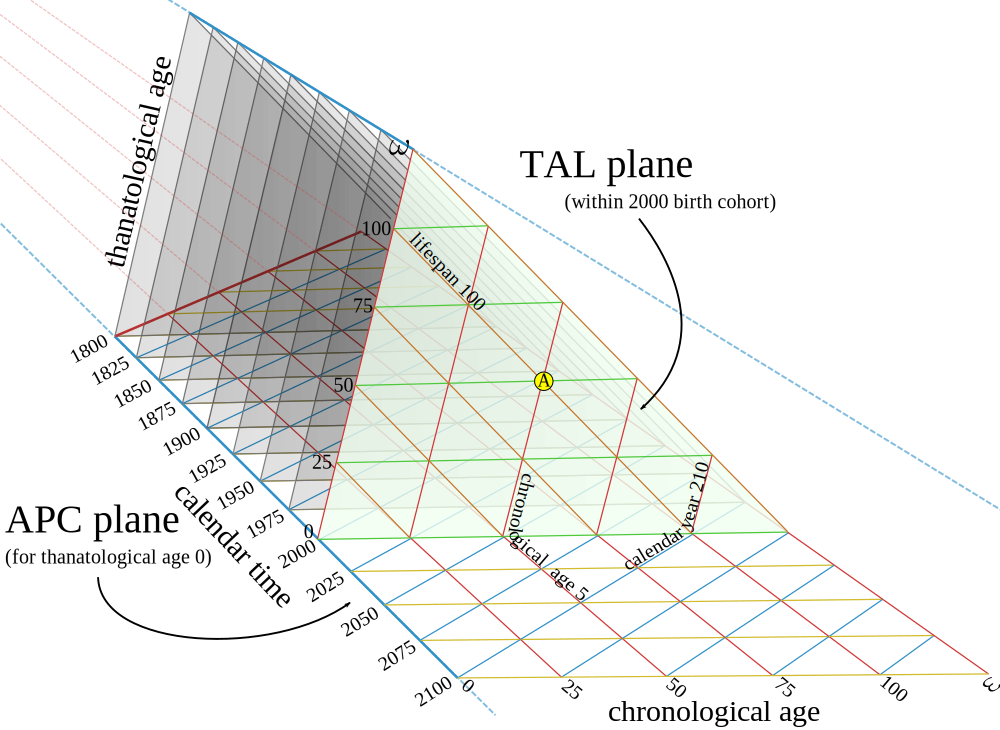
\includegraphics[scale=.8]{Figures/buildTAL5.pdf}
\end{center}
\end{frame}

%-------------------

%\begin{frame}
%\frametitle{APC can reveal patterns}
%\begin{center}
%\includegraphics[trim 100 100 300
%300,scale=.5]{Figures/Perozzo1000px_cropped_adj.png}
%\end{center}
%\end{frame}

%-------------------

\begin{frame}
\frametitle{dimensions and states}
\vspace{-10em}
\begin{center}
\hspace*{-6cm}\includegraphics[scale=.7]{Figures/prism.jpg}
\end{center}
\end{frame}

%------------------------------
% Think of images to use here %
%------------------------------
\begin{frame}
\frametitle{So why more planes?}
\normalsize
\begin{itemize}[<+->]
  \item to uncover more patterns  % magnifying glass
  \item to improve measurement    % calipers
  \item to make better models     % icons of birth death marriage boxes and
  % arrows
  \item to understand processes   % person thinking?
\end{itemize}
\end{frame}


%----------------------------------

\begin{frame}
\frametitle{You should}
\normalsize
\begin{itemize}[<+->]
  \item make an origami tetrahedron and label its edges with the demographic
  time measures
  \item visualize data structured in this way ASAP, because you might see new
  and exciting things
\end{itemize}
\end{frame}

%----------------------------------

\begin{frame}
\frametitle{Thanks!}
\vspace{-4em}
\begin{center}
\includegraphics[scale=1.7]{Figures/TetraHedronEdgesOnly.pdf}
\end{center}
\end{frame}

%---------------------------------
% Extra material                 %
%---------------------------------
\begin{frame}
\frametitle{An example inquiry}
\normalsize
\begin{itemize}[<+->]
  \item compare end-of-life trajectories for several birth cohorts (1905 - 1925)
  \item HRS (Rand), waves 1-11 (years 1992-2012)
  \item use TAL plane to uncover patterns that APC hides
  \item this example: prevalence of poor self-reported health
\end{itemize}
\end{frame}

%---------------------------

\begin{frame}
\frametitle{1905 cohort}
\vspace{-4em}
\begin{center}
\includegraphics[scale=1]{Figures/srhpoor1905.pdf}
\end{center}
\end{frame}

%---------------------------

\begin{frame}
\frametitle{1910 cohort, looking pretty similar}
\vspace{-4em}
\begin{center}
\includegraphics[scale=1]{Figures/srhpoor1910.pdf}
\end{center}
\end{frame}

%---------------------------

\begin{frame}
\frametitle{1915 cohort, looking pretty similar}
\vspace{-4em}
\begin{center}
\includegraphics[scale=1]{Figures/srhpoor1915.pdf}
\end{center}
\end{frame}

%---------------------------

\begin{frame}
\frametitle{1920 cohort, looking pretty similar}
\vspace{-4em}
\begin{center}
\includegraphics[scale=1]{Figures/srhpoor1920.pdf}
\end{center}
\end{frame}

%---------------------------

\begin{frame}
\frametitle{1925 cohort, looking pretty similar}
\vspace{-4em}
\begin{center}
\includegraphics[scale=1]{Figures/srhpoor1925.pdf}
\end{center}
\end{frame}

%----------------------------------

\begin{frame}
\frametitle{So why more planes?}
\normalsize
\begin{itemize}[<+->]
  \item easier to detect patterns
  \item to better understand the relationships between the measures of
  demographic time
\end{itemize}
\end{frame}

%%%%%%%%%%%%%%%%%%%%%%%%%%%%%%%%%%
%%	End of the document			%%
%%%%%%%%%%%%%%%%%%%%%%%%%%%%%%%%%%
\end{document}










